\documentclass[12pt,a4paper]{article}
\usepackage{amsmath,amscd,amsbsy,amssymb,latexsym,url,bm,amsthm}
\usepackage{epsfig,graphicx,subfigure}
\usepackage{enumitem,balance}
\usepackage{wrapfig}
\usepackage{mathrsfs,euscript}
\usepackage[usenames]{xcolor}
\usepackage{hyperref}
\usepackage[vlined,ruled,linesnumbered]{algorithm2e}
\hypersetup{colorlinks=true,linkcolor=black}

\newtheorem{theorem}{Theorem}
\newtheorem{lemma}[theorem]{Lemma}
\newtheorem{proposition}[theorem]{Proposition}
\newtheorem{corollary}[theorem]{Corollary}
\newtheorem{exercise}{Exercise}
\newtheorem*{solution}{Solution}
\newtheorem{definition}{Definition}
\theoremstyle{definition}

\renewcommand{\thefootnote}{\fnsymbol{footnote}}

\newcommand{\postscript}[2]
 {\setlength{\epsfxsize}{#2\hsize}
  \centerline{\epsfbox{#1}}}

\renewcommand{\baselinestretch}{1.0}

\setlength{\oddsidemargin}{-0.365in}
\setlength{\evensidemargin}{-0.365in}
\setlength{\topmargin}{-0.3in}
\setlength{\headheight}{0in}
\setlength{\headsep}{0in}
\setlength{\textheight}{10.1in}
\setlength{\textwidth}{7in}
\makeatletter \renewenvironment{proof}[1][Proof] {\par\pushQED{\qed}\normalfont\topsep6\p@\@plus6\p@\relax\trivlist\item[\hskip\labelsep\bfseries#1\@addpunct{.}]\ignorespaces}{\popQED\endtrivlist\@endpefalse} \makeatother
\makeatletter
\renewenvironment{solution}[1][Solution] {\par\pushQED{\qed}\normalfont\topsep6\p@\@plus6\p@\relax\trivlist\item[\hskip\labelsep\bfseries#1\@addpunct{.}]\ignorespaces}{\popQED\endtrivlist\@endpefalse} \makeatother

\begin{document}
\noindent

%========================================================================
\noindent\framebox[\linewidth]{\shortstack[c]{
\Large{\textbf{Lab02-Divide and Conquer}}\vspace{1mm}\\
CS214-Algorithm and Complexity, Xiaofeng Gao, Spring 2021.}}
\begin{center}
\footnotesize{\color{red}$*$ If there is any problem, please contact TA Haolin Zhou. }

\footnotesize{\color{blue}$*$ Name:Yanjie Ze  \quad Student ID:519021910706 \quad Email: zeyanjie@sjtu.edu.cn}
\end{center}

\begin{enumerate}
\item
    \textit{Recurrence examples.} Give asymptotic upper and lower bounds for $T(n)$ in each of the following recurrences. Assume that $T(n)$ is constant for sufficiently small $n$. Make your bounds as tight as possible.
\begin{enumerate}
	\item $T(n)=4 T(n / 3)+n \log n$
	\item $T(n)=4 T(n / 2)+n^{2} \sqrt{n}$
	\item $T(n)=T(n-1)+n$	
	\item $T(n)=2T(\lfloor \sqrt n\rfloor)+\log n$
\end{enumerate}
\begin{solution}
\begin{enumerate}
% 第一题
\item 
Because $n<nlogn<n^2$, and we denote: 
$$T_1(n)=4 T(n / 3)+n$$
$$T_2(n)=4 T(n / 3)+n^2$$
Based on Master Theorem, we have:
$$
T_1(n)=O(n^{log_34})
$$
$$
T_2(n)=O(n^2)
$$
Therefore:
$$
T(n)=O(n^2), T(n)=\Omega(n^{log_34})
$$
\item
 $$
 T(n)=4 T(n / 2)+n^{2} \sqrt{n}=4 T(n / 2)+n^{\frac{5}{2}} 
 $$
 Based on Master Theorem, $a=4, b=2, d=\frac{5}{2}$,we have:
 
 $$
 T(n) = O(n^\frac{5}{2})
 $$
 
 \item
 $$
 \displaystyle T(n)=\sum_{i=1}^ni+T(0) = \frac{n^2+n}{2}+T(0)
 $$
 Thus:
 $$
 T(n)=\Omega(n^2)
 $$
 
 \item
Assume $n=2^{2^k}$, then $k=log_2(log_2n)$. 

$$
T(2^{2^k}) = 2T(2^{2^{k-1}})+2^klog2
$$
$$
\frac{T(2^{2^k})}{2^k} = \frac{T(2^{2^{k-1}})}{2^{k-1}}+log2
$$
Thus we can sum them together and get:
$$
 \frac{T(2^{2^k})}{2^k} = (k-1)log2 + T(2)
$$
Multiply both sides by $2^k$ and then replace $k$ by $n$:
$$
T(n) = log2\cdot log_2n\cdot log_2(log_2n)+ T(2)\cdot log_2n
$$
Therefore:
$$
T(n) = \Theta(logn\cdot log(logn))
$$

\end{enumerate}
\end{solution}
\item
\textit{Divide-and-conquer.} Given an integer array $A[1..n]$ and two integers $lower \le upper$, design an algorithm using \textbf{divide-and-conquer} method to count the number of ranges $(i,j)$ ($1 \leq i \leq j \leq n$) satisfying
$$
    lower \leq \sum_{k=i}^{j}{A[k]} \leq upper.
$$
\textbf{Example:}

Given $A = [1,-1,2]$, $lower = 1$, $upper = 2$, return 4.

The resulting four ranges are $(1,1)$, $(3,3)$, $(2,3)$ and $(1,3)$.

\begin{enumerate}
\item
Complete the implementation in the provided C/C++ source code {\color{blue}(The source code \emph{Code-Range.cpp} is attached on the course webpage)}.
\item
Write a recurrence for the running time of the algorithm and solve it by recurrence tree {\color{blue}(You can modify the figure sources \emph{Fig-RecurrenceTree.vsdx} or \emph{Fig-RecurrenceTree.pptx} to illustrate your derivation)}.
\item
Can we use the Master Theorem to solve the recurrence above? Please explain your answer.
\end{enumerate}

%第二题
\begin{solution}
\begin{enumerate}
\item
$$
T(n) = 2T(\frac{n}{2}) + nlogn
$$
\end{enumerate}
\end{solution}
\item
\textit{Transposition Sorting Network.} A comparison network is a \textbf{transposition network}  if each comparator connects adjacent lines, as in the network in Fig. ~\ref{Fig-Transposition}.

\begin{figure}[htbp]
    \centering
    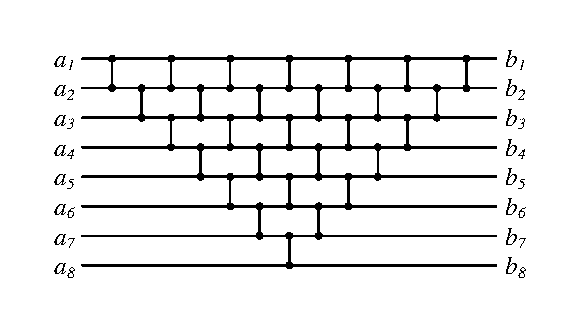
\includegraphics[width=0.4\textwidth]{Fig-Transposition.pdf}
    \caption{A Transposition Network Example}\label{Fig-Transposition}
\end{figure}

\begin{enumerate}
\item Prove that a transposition network with $n$ inputs is a sorting network if and only if it sorts the sequence $\langle n, n-1, \cdots, 1 \rangle$. {\color{blue}(Hint: Use an induction argument analogous to the \emph{Domain Conversion Lemma}.)}
\item {\color{red}{(Optional Sub-question with Bonus)}} Given any $n \in \mathbb{N}$, write a program using Tkinter in Python to draw a figure similar to Fig.~\ref{Fig-Transposition} with $n$ input wires.
\end{enumerate}
\end{enumerate}
%\begin{solution}
%response...
%\end{solution}
%========================================================================
\end{document}
